% Options for packages loaded elsewhere
\PassOptionsToPackage{unicode}{hyperref}
\PassOptionsToPackage{hyphens}{url}
%
\documentclass[
]{article}
\usepackage{amsmath,amssymb}
\usepackage{lmodern}
\usepackage{ifxetex,ifluatex}
\ifnum 0\ifxetex 1\fi\ifluatex 1\fi=0 % if pdftex
  \usepackage[T1]{fontenc}
  \usepackage[utf8]{inputenc}
  \usepackage{textcomp} % provide euro and other symbols
\else % if luatex or xetex
  \usepackage{unicode-math}
  \defaultfontfeatures{Scale=MatchLowercase}
  \defaultfontfeatures[\rmfamily]{Ligatures=TeX,Scale=1}
\fi
% Use upquote if available, for straight quotes in verbatim environments
\IfFileExists{upquote.sty}{\usepackage{upquote}}{}
\IfFileExists{microtype.sty}{% use microtype if available
  \usepackage[]{microtype}
  \UseMicrotypeSet[protrusion]{basicmath} % disable protrusion for tt fonts
}{}
\makeatletter
\@ifundefined{KOMAClassName}{% if non-KOMA class
  \IfFileExists{parskip.sty}{%
    \usepackage{parskip}
  }{% else
    \setlength{\parindent}{0pt}
    \setlength{\parskip}{6pt plus 2pt minus 1pt}}
}{% if KOMA class
  \KOMAoptions{parskip=half}}
\makeatother
\usepackage{xcolor}
\IfFileExists{xurl.sty}{\usepackage{xurl}}{} % add URL line breaks if available
\IfFileExists{bookmark.sty}{\usepackage{bookmark}}{\usepackage{hyperref}}
\hypersetup{
  pdftitle={01 Intro to the tidyverse},
  pdfauthor={Joschka Schwarz},
  hidelinks,
  pdfcreator={LaTeX via pandoc}}
\urlstyle{same} % disable monospaced font for URLs
\usepackage[margin=1in]{geometry}
\usepackage{color}
\usepackage{fancyvrb}
\newcommand{\VerbBar}{|}
\newcommand{\VERB}{\Verb[commandchars=\\\{\}]}
\DefineVerbatimEnvironment{Highlighting}{Verbatim}{commandchars=\\\{\}}
% Add ',fontsize=\small' for more characters per line
\usepackage{framed}
\definecolor{shadecolor}{RGB}{248,248,248}
\newenvironment{Shaded}{\begin{snugshade}}{\end{snugshade}}
\newcommand{\AlertTok}[1]{\textcolor[rgb]{0.94,0.16,0.16}{#1}}
\newcommand{\AnnotationTok}[1]{\textcolor[rgb]{0.56,0.35,0.01}{\textbf{\textit{#1}}}}
\newcommand{\AttributeTok}[1]{\textcolor[rgb]{0.77,0.63,0.00}{#1}}
\newcommand{\BaseNTok}[1]{\textcolor[rgb]{0.00,0.00,0.81}{#1}}
\newcommand{\BuiltInTok}[1]{#1}
\newcommand{\CharTok}[1]{\textcolor[rgb]{0.31,0.60,0.02}{#1}}
\newcommand{\CommentTok}[1]{\textcolor[rgb]{0.56,0.35,0.01}{\textit{#1}}}
\newcommand{\CommentVarTok}[1]{\textcolor[rgb]{0.56,0.35,0.01}{\textbf{\textit{#1}}}}
\newcommand{\ConstantTok}[1]{\textcolor[rgb]{0.00,0.00,0.00}{#1}}
\newcommand{\ControlFlowTok}[1]{\textcolor[rgb]{0.13,0.29,0.53}{\textbf{#1}}}
\newcommand{\DataTypeTok}[1]{\textcolor[rgb]{0.13,0.29,0.53}{#1}}
\newcommand{\DecValTok}[1]{\textcolor[rgb]{0.00,0.00,0.81}{#1}}
\newcommand{\DocumentationTok}[1]{\textcolor[rgb]{0.56,0.35,0.01}{\textbf{\textit{#1}}}}
\newcommand{\ErrorTok}[1]{\textcolor[rgb]{0.64,0.00,0.00}{\textbf{#1}}}
\newcommand{\ExtensionTok}[1]{#1}
\newcommand{\FloatTok}[1]{\textcolor[rgb]{0.00,0.00,0.81}{#1}}
\newcommand{\FunctionTok}[1]{\textcolor[rgb]{0.00,0.00,0.00}{#1}}
\newcommand{\ImportTok}[1]{#1}
\newcommand{\InformationTok}[1]{\textcolor[rgb]{0.56,0.35,0.01}{\textbf{\textit{#1}}}}
\newcommand{\KeywordTok}[1]{\textcolor[rgb]{0.13,0.29,0.53}{\textbf{#1}}}
\newcommand{\NormalTok}[1]{#1}
\newcommand{\OperatorTok}[1]{\textcolor[rgb]{0.81,0.36,0.00}{\textbf{#1}}}
\newcommand{\OtherTok}[1]{\textcolor[rgb]{0.56,0.35,0.01}{#1}}
\newcommand{\PreprocessorTok}[1]{\textcolor[rgb]{0.56,0.35,0.01}{\textit{#1}}}
\newcommand{\RegionMarkerTok}[1]{#1}
\newcommand{\SpecialCharTok}[1]{\textcolor[rgb]{0.00,0.00,0.00}{#1}}
\newcommand{\SpecialStringTok}[1]{\textcolor[rgb]{0.31,0.60,0.02}{#1}}
\newcommand{\StringTok}[1]{\textcolor[rgb]{0.31,0.60,0.02}{#1}}
\newcommand{\VariableTok}[1]{\textcolor[rgb]{0.00,0.00,0.00}{#1}}
\newcommand{\VerbatimStringTok}[1]{\textcolor[rgb]{0.31,0.60,0.02}{#1}}
\newcommand{\WarningTok}[1]{\textcolor[rgb]{0.56,0.35,0.01}{\textbf{\textit{#1}}}}
\usepackage{graphicx}
\makeatletter
\def\maxwidth{\ifdim\Gin@nat@width>\linewidth\linewidth\else\Gin@nat@width\fi}
\def\maxheight{\ifdim\Gin@nat@height>\textheight\textheight\else\Gin@nat@height\fi}
\makeatother
% Scale images if necessary, so that they will not overflow the page
% margins by default, and it is still possible to overwrite the defaults
% using explicit options in \includegraphics[width, height, ...]{}
\setkeys{Gin}{width=\maxwidth,height=\maxheight,keepaspectratio}
% Set default figure placement to htbp
\makeatletter
\def\fps@figure{htbp}
\makeatother
\setlength{\emergencystretch}{3em} % prevent overfull lines
\providecommand{\tightlist}{%
  \setlength{\itemsep}{0pt}\setlength{\parskip}{0pt}}
\setcounter{secnumdepth}{-\maxdimen} % remove section numbering
\ifluatex
  \usepackage{selnolig}  % disable illegal ligatures
\fi

\title{01 Intro to the tidyverse}
\author{Joschka Schwarz}
\date{2021-04}

\begin{document}
\maketitle

{
\setcounter{tocdepth}{3}
\tableofcontents
}
\hypertarget{my-first-post}{%
\section{My first post}\label{my-first-post}}

My name is Sharon Nisha Thiruvarul Duai. My immatricultain number is
21653851 . Iam currently doing my masters in ``Elektrotechnik''

\begin{Shaded}
\begin{Highlighting}[]
\FunctionTok{library}\NormalTok{(readxl)}
\FunctionTok{library}\NormalTok{(tidyverse)}
\FunctionTok{library}\NormalTok{(lubridate)}

\CommentTok{\# by automatically detecting a common column, if any ...}
\NormalTok{bikes\_tbl      }\OtherTok{\textless{}{-}} \FunctionTok{read\_excel}\NormalTok{(}\AttributeTok{path =} \StringTok{"C:/Users/ctaru/Desktop/businessdatascience/ds\_data/ds\_data/01\_bike\_sales/01\_raw\_data/bikes.xlsx"}\NormalTok{)}
\NormalTok{orderlines\_tbl }\OtherTok{\textless{}{-}} \FunctionTok{read\_excel}\NormalTok{(}\StringTok{"C:/Users/ctaru/Desktop/businessdatascience/ds\_data/ds\_data/01\_bike\_sales/01\_raw\_data/orderlines.xlsx"}\NormalTok{)}
\NormalTok{bikeshops\_tbl }\OtherTok{\textless{}{-}}\FunctionTok{read\_excel}\NormalTok{(}\StringTok{"C:/Users/ctaru/Desktop/businessdatascience/ds\_data/ds\_data/01\_bike\_sales/01\_raw\_data/bikeshops.xlsx"}\NormalTok{)}



\NormalTok{bike\_orderlines\_joined\_tbl }\OtherTok{\textless{}{-}}\NormalTok{ orderlines\_tbl }\SpecialCharTok{\%\textgreater{}\%}
        \FunctionTok{left\_join}\NormalTok{(bikes\_tbl, }\AttributeTok{by =} \FunctionTok{c}\NormalTok{(}\StringTok{"product.id"} \OtherTok{=} \StringTok{"bike.id"}\NormalTok{)) }\SpecialCharTok{\%\textgreater{}\%}
        \FunctionTok{left\_join}\NormalTok{(bikeshops\_tbl, }\AttributeTok{by =} \FunctionTok{c}\NormalTok{(}\StringTok{"customer.id"} \OtherTok{=} \StringTok{"bikeshop.id"}\NormalTok{))}



\NormalTok{copy\_bike\_orderlines\_joined\_tbl}\OtherTok{\textless{}{-}}\NormalTok{bike\_orderlines\_joined\_tbl}



\NormalTok{bike\_orderlines\_wrangled\_tbl }\OtherTok{\textless{}{-}}\NormalTok{ copy\_bike\_orderlines\_joined\_tbl }\SpecialCharTok{\%\textgreater{}\%}
  \CommentTok{\# 5.1 Separate category name}
  \FunctionTok{separate}\NormalTok{(}\AttributeTok{col    =}\NormalTok{ location,}
           \AttributeTok{into   =} \FunctionTok{c}\NormalTok{(}\StringTok{"city"}\NormalTok{, }\StringTok{"state"}\NormalTok{),}
           \AttributeTok{sep    =} \StringTok{","}\NormalTok{) }\SpecialCharTok{\%\textgreater{}\%}
\CommentTok{\#didnot want to convert dots to dashes for simplicity}
                    \CommentTok{\#set\_names(names(.) \%\textgreater{}\% str\_replace\_all("\textbackslash{}\textbackslash{}.", "\_"))}
  \CommentTok{\# 5.2 Add the total price (price * quantity) }
  \CommentTok{\# Add a column to a tibble that uses a formula{-}style calculation of other columns}
  \FunctionTok{mutate}\NormalTok{(}\AttributeTok{total.price =}\NormalTok{ price }\SpecialCharTok{*}\NormalTok{ quantity)}



\NormalTok{sales\_by\_loc\_tbl }\OtherTok{\textless{}{-}}\NormalTok{bike\_orderlines\_wrangled\_tbl}\SpecialCharTok{\%\textgreater{}\%}
\CommentTok{\#Sales by state }

  \CommentTok{\# Select columns}
  \FunctionTok{select}\NormalTok{(state, total.price) }\SpecialCharTok{\%\textgreater{}\%} 
  \FunctionTok{group\_by}\NormalTok{(state) }\SpecialCharTok{\%\textgreater{}\%} 
  \FunctionTok{summarize}\NormalTok{(}\AttributeTok{sales =} \FunctionTok{sum}\NormalTok{(total.price)) }\SpecialCharTok{\%\textgreater{}\%}
  \FunctionTok{mutate}\NormalTok{(}\AttributeTok{sales\_text =}\NormalTok{ scales}\SpecialCharTok{::}\FunctionTok{dollar}\NormalTok{(sales, }\AttributeTok{big.mark =} \StringTok{"."}\NormalTok{, }
                                     \AttributeTok{decimal.mark =} \StringTok{","}\NormalTok{, }
                                     \AttributeTok{prefix =} \StringTok{""}\NormalTok{, }
                                     \AttributeTok{suffix =} \StringTok{" €"}\NormalTok{))}

\NormalTok{intermediate\_table}\OtherTok{\textless{}{-}}\NormalTok{bike\_orderlines\_wrangled\_tbl}

\NormalTok{sales\_by\_loc\_tbl}
\end{Highlighting}
\end{Shaded}

\begin{verbatim}
## # A tibble: 12 x 3
##    state                               sales sales_text  
##    <chr>                               <dbl> <chr>       
##  1 " Baden-Württemberg"              6521090 6.521.090 € 
##  2 " Bavaria"                        6742819 6.742.819 € 
##  3 " Berlin"                         1128433 1.128.433 € 
##  4 " Bremen"                        10653499 10.653.499 €
##  5 " Hamburg"                        3874756 3.874.756 € 
##  6 " Hesse"                          1558901 1.558.901 € 
##  7 " Lower Saxony"                   4107115 4.107.115 € 
##  8 " Mecklenburg-Western Pomerania"   618974 618.974 €   
##  9 " North Rhine-Westphalia"        21200613 21.200.613 €
## 10 " Saxony"                         2230245 2.230.245 € 
## 11 " Saxony-Anhalt"                   569614 569.614 €   
## 12 " Schleswig-Holstein"             3224749 3.224.749 €
\end{verbatim}

\begin{Shaded}
\begin{Highlighting}[]
  \CommentTok{\# Step 2 {-} Visualize}
 
\NormalTok{  sales\_by\_loc\_tbl }\SpecialCharTok{\%\textgreater{}\%}
  

  \FunctionTok{ggplot}\NormalTok{(}\FunctionTok{aes}\NormalTok{(}\AttributeTok{x =}\NormalTok{ state, }\AttributeTok{y =}\NormalTok{ sales)) }\SpecialCharTok{+}


  \CommentTok{\# Geometries}
  \FunctionTok{geom\_col}\NormalTok{(}\AttributeTok{fill =} \StringTok{"\#2DC6D6"}\NormalTok{) }\SpecialCharTok{+} \CommentTok{\# Use geom\_col for a bar plot}
  \FunctionTok{geom\_label}\NormalTok{(}\FunctionTok{aes}\NormalTok{(}\AttributeTok{label =}\NormalTok{ sales\_text)) }\SpecialCharTok{+} \CommentTok{\# Adding labels to the bars}
  \FunctionTok{geom\_smooth}\NormalTok{(}\AttributeTok{method =} \StringTok{"lm"}\NormalTok{, }\AttributeTok{se =} \ConstantTok{FALSE}\NormalTok{) }\SpecialCharTok{+} \CommentTok{\# Adding a trendline}


  \FunctionTok{scale\_y\_continuous}\NormalTok{(}\AttributeTok{labels =}\NormalTok{ scales}\SpecialCharTok{::}\FunctionTok{dollar\_format}\NormalTok{(}\AttributeTok{big.mark =} \StringTok{"."}\NormalTok{, }
                                                    \AttributeTok{decimal.mark =} \StringTok{","}\NormalTok{, }
                                                    \AttributeTok{prefix =} \StringTok{""}\NormalTok{, }
                                                    \AttributeTok{suffix =} \StringTok{" €"}\NormalTok{))}\SpecialCharTok{+}
  \FunctionTok{theme}\NormalTok{(}\AttributeTok{axis.text.x =} \FunctionTok{element\_text}\NormalTok{(}\AttributeTok{size=}\DecValTok{10}\NormalTok{,}\AttributeTok{angle =} \DecValTok{45}\NormalTok{, }\AttributeTok{hjust =} \DecValTok{1}\NormalTok{))}\SpecialCharTok{+}\CommentTok{\#added size of x text and angled}
  \FunctionTok{theme}\NormalTok{(}\AttributeTok{axis.text.y =} \FunctionTok{element\_text}\NormalTok{(}\AttributeTok{size=}\DecValTok{10}\NormalTok{, }\AttributeTok{hjust =} \DecValTok{1}\NormalTok{))}\CommentTok{\#added extra line for y text size incrementno need of angle}
\end{Highlighting}
\end{Shaded}

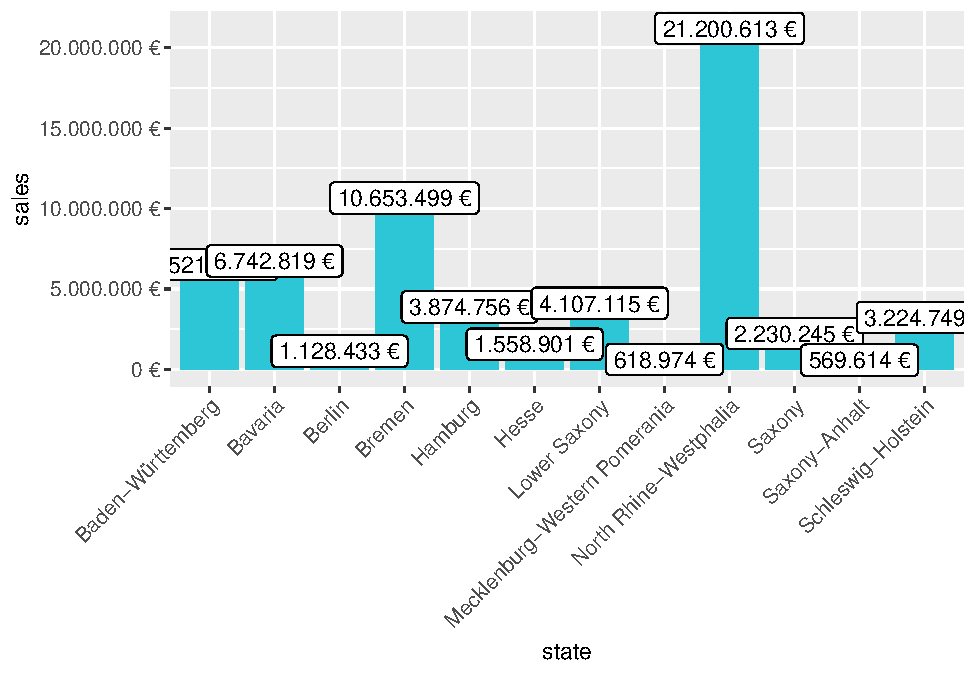
\includegraphics{01_tidyverse_files/figure-latex/unnamed-chunk-2-1.pdf}

\begin{Shaded}
\begin{Highlighting}[]
  \FunctionTok{labs}\NormalTok{(}
    \AttributeTok{title    =} \StringTok{"Revenue by location"}\NormalTok{,}
    \AttributeTok{subtitle =} \StringTok{""}\NormalTok{,}
    \AttributeTok{x =} \StringTok{""}\NormalTok{, }\CommentTok{\# Override defaults for x and y}
    \AttributeTok{y =} \StringTok{"Revenue"}
\NormalTok{  )}
\end{Highlighting}
\end{Shaded}

\begin{verbatim}
## $x
## [1] ""
## 
## $y
## [1] "Revenue"
## 
## $title
## [1] "Revenue by location"
## 
## $subtitle
## [1] ""
## 
## attr(,"class")
## [1] "labels"
\end{verbatim}

newxt exercise

\begin{Shaded}
\begin{Highlighting}[]
\DocumentationTok{\#\#\#\#\#\#this part is to be able to plot 2 parameters}

\FunctionTok{library}\NormalTok{(readxl)}
\FunctionTok{library}\NormalTok{(tidyverse)}
\FunctionTok{library}\NormalTok{(lubridate)}

\NormalTok{sales\_by\_yea\_tbl }\OtherTok{\textless{}{-}}\NormalTok{intermediate\_table}\SpecialCharTok{\%\textgreater{}\%} 

  \FunctionTok{mutate}\NormalTok{(}\AttributeTok{total.price =}\NormalTok{ price }\SpecialCharTok{*}\NormalTok{ quantity) }\SpecialCharTok{\%\textgreater{}\%}
\CommentTok{\# 6.1 Sales by Year {-}{-}{-}{-}}
  \FunctionTok{mutate}\NormalTok{(}\AttributeTok{year=}\FunctionTok{year}\NormalTok{(order.date))}\SpecialCharTok{\%\textgreater{}\%}
  \CommentTok{\# Select columns}
  \FunctionTok{select}\NormalTok{(state,year,total.price)}\SpecialCharTok{\%\textgreater{}\%} 
  \FunctionTok{group\_by}\NormalTok{(state) }

\DocumentationTok{\#\#\#\#\#\#\#\#\#\#\#\#\#\#\#\#\#\#\#\#\#\#}

\NormalTok{ hamburg\_tbl }\OtherTok{\textless{}{-}}\NormalTok{sales\_by\_yea\_tbl}\SpecialCharTok{\%\textgreater{}\%}
  \FunctionTok{select}\NormalTok{(year, total.price, state)}\SpecialCharTok{\%\textgreater{}\%}
 
 \FunctionTok{group\_by}\NormalTok{(year,state)}\DocumentationTok{\#\#\#\#\#each year each state how much sales has now been grouped}
\NormalTok{hamburg\_tbl}
\end{Highlighting}
\end{Shaded}

\begin{verbatim}
## # A tibble: 15,644 x 3
## # Groups:   year, state [60]
##     year total.price state               
##    <dbl>       <dbl> <chr>               
##  1  2015        3119 " Hamburg"          
##  2  2015        5359 " Hamburg"          
##  3  2015        2729 " Bremen"           
##  4  2015        1749 " Bremen"           
##  5  2015        1219 " Baden-Württemberg"
##  6  2015        1359 " Baden-Württemberg"
##  7  2015        2529 " Baden-Württemberg"
##  8  2015        1559 " Baden-Württemberg"
##  9  2015        3899 " Baden-Württemberg"
## 10  2015        6629 " Bavaria"          
## # ... with 15,634 more rows
\end{verbatim}

\begin{Shaded}
\begin{Highlighting}[]
\DocumentationTok{\#\#\#\#\#\#\#\#\#\#\#\#\#\#\#\#\#\#\#\#\#\#\#\#\#\#\#\#\#\#}
\NormalTok{  hamburg\_tbl}\SpecialCharTok{\%\textgreater{}\%}
  \CommentTok{\# Set up x, y, fill}
  \FunctionTok{ggplot}\NormalTok{(}\FunctionTok{aes}\NormalTok{(}\AttributeTok{x =}\NormalTok{ year, }\AttributeTok{y =}\NormalTok{ total.price, }\AttributeTok{fill =}\NormalTok{ state)) }\SpecialCharTok{+}

  \CommentTok{\# Geometries}
  \FunctionTok{geom\_col}\NormalTok{() }\SpecialCharTok{+} \CommentTok{\# Run up to here to get a stacked bar plot}

  \CommentTok{\# Facet}
  \FunctionTok{facet\_wrap}\NormalTok{(}\SpecialCharTok{\textasciitilde{}}\NormalTok{ state) }\SpecialCharTok{+}

  \CommentTok{\# Formatting}
  \FunctionTok{scale\_y\_continuous}\NormalTok{(}\AttributeTok{labels =}\NormalTok{ scales}\SpecialCharTok{::}\FunctionTok{dollar\_format}\NormalTok{(}\AttributeTok{big.mark =} \StringTok{"."}\NormalTok{, }
                                                    \AttributeTok{decimal.mark =} \StringTok{","}\NormalTok{, }
                                                    \AttributeTok{prefix =} \StringTok{""}\NormalTok{, }
                                                    \AttributeTok{suffix =} \StringTok{" €"}\NormalTok{)) }\SpecialCharTok{+}
  \FunctionTok{labs}\NormalTok{(}
    \AttributeTok{title =} \StringTok{"Total sale per month based on state"}\NormalTok{,}
    \AttributeTok{subtitle =} \StringTok{"Each product category has an upward trend"}\NormalTok{,}
    \AttributeTok{fill =} \StringTok{"Main category"} \CommentTok{\# Changes the legend name}
\NormalTok{  )}
\end{Highlighting}
\end{Shaded}

\includegraphics{01_tidyverse_files/figure-latex/plot-1.pdf}

Results:North Rhine-Westphalia has the highest sales

\end{document}
